\begin{figure*}[t]
\begin{minipage}[b]{0.32\linewidth}
\centering
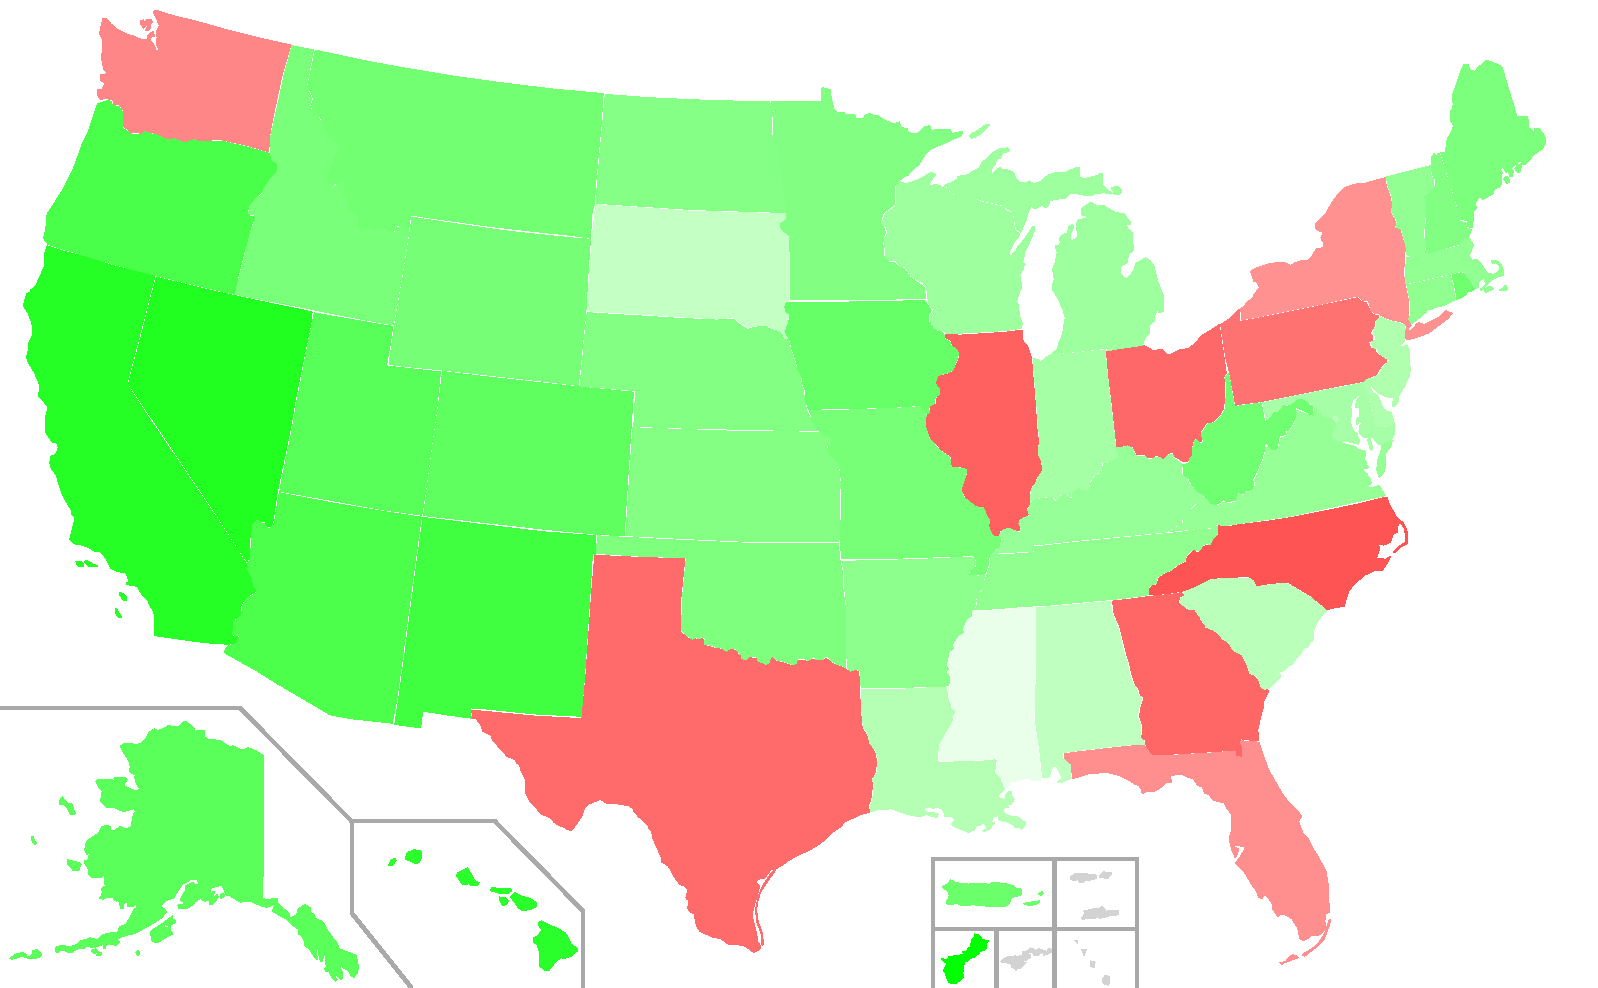
\includegraphics[width=53mm]{./images/ca.pdf}
\caption{Followers of California}
\label{fig:state-ca}
\end{minipage}
\hspace{2mm}
\begin{minipage}[b]{0.32\linewidth}
\centering
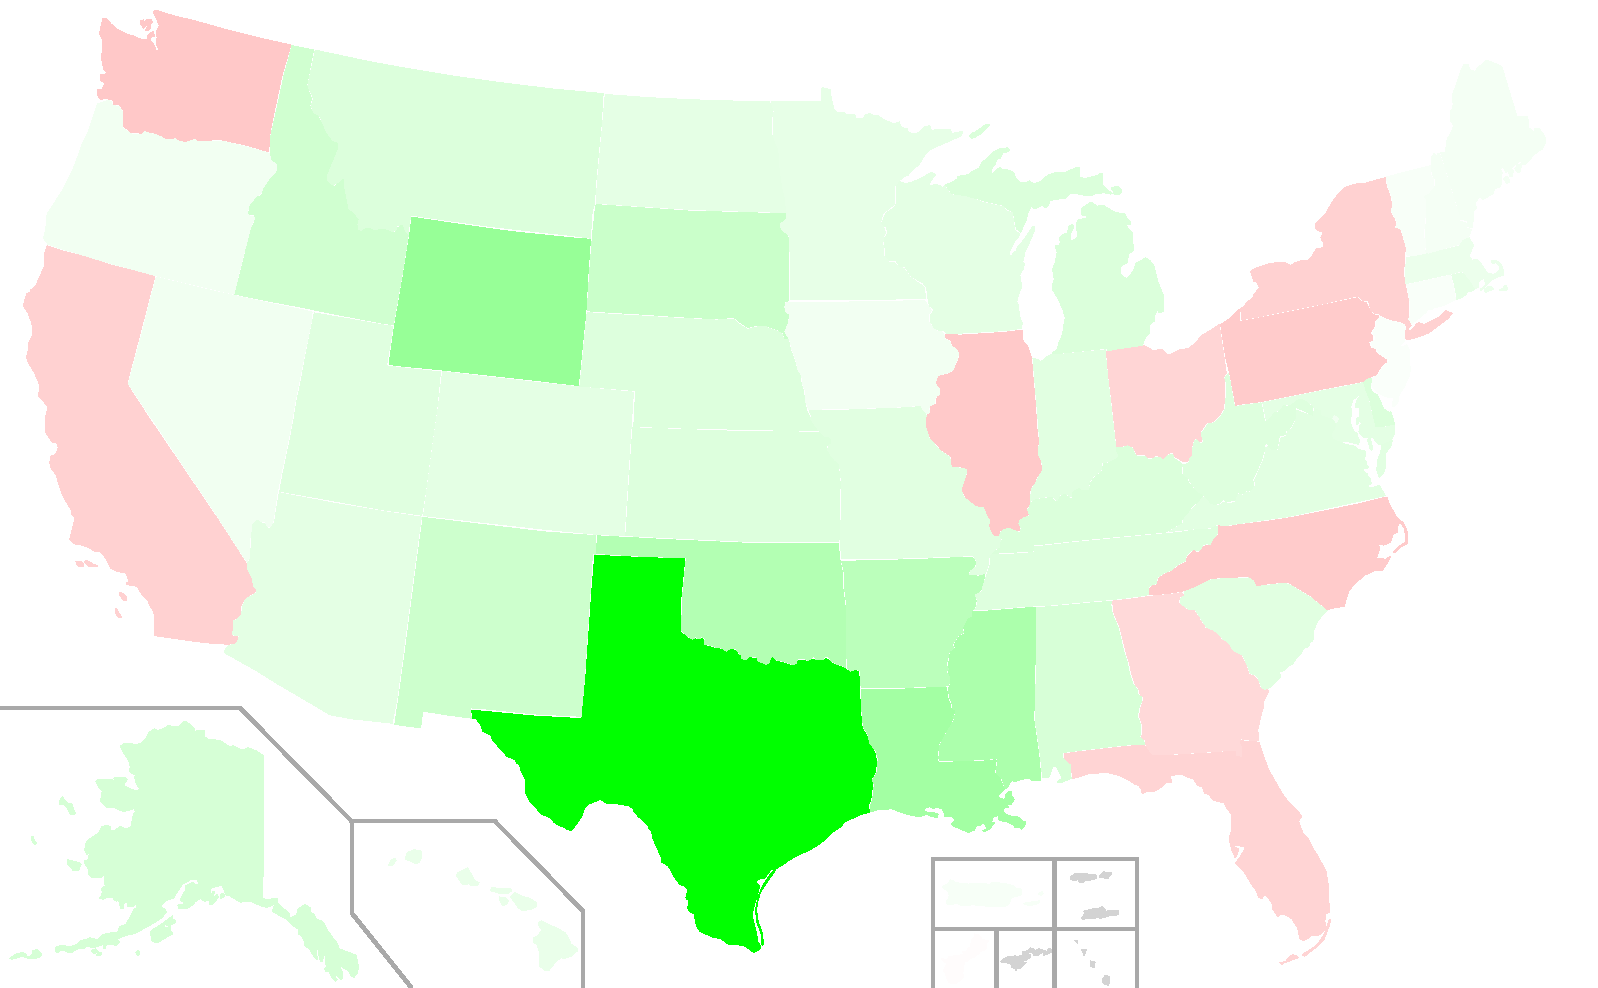
\includegraphics[width=53mm]{./images/tx.pdf}
\caption{Followers of Texas}
\label{fig:state-tx}
\end{minipage}
\hspace{2mm}
\begin{minipage}[b]{0.32\linewidth}
\centering
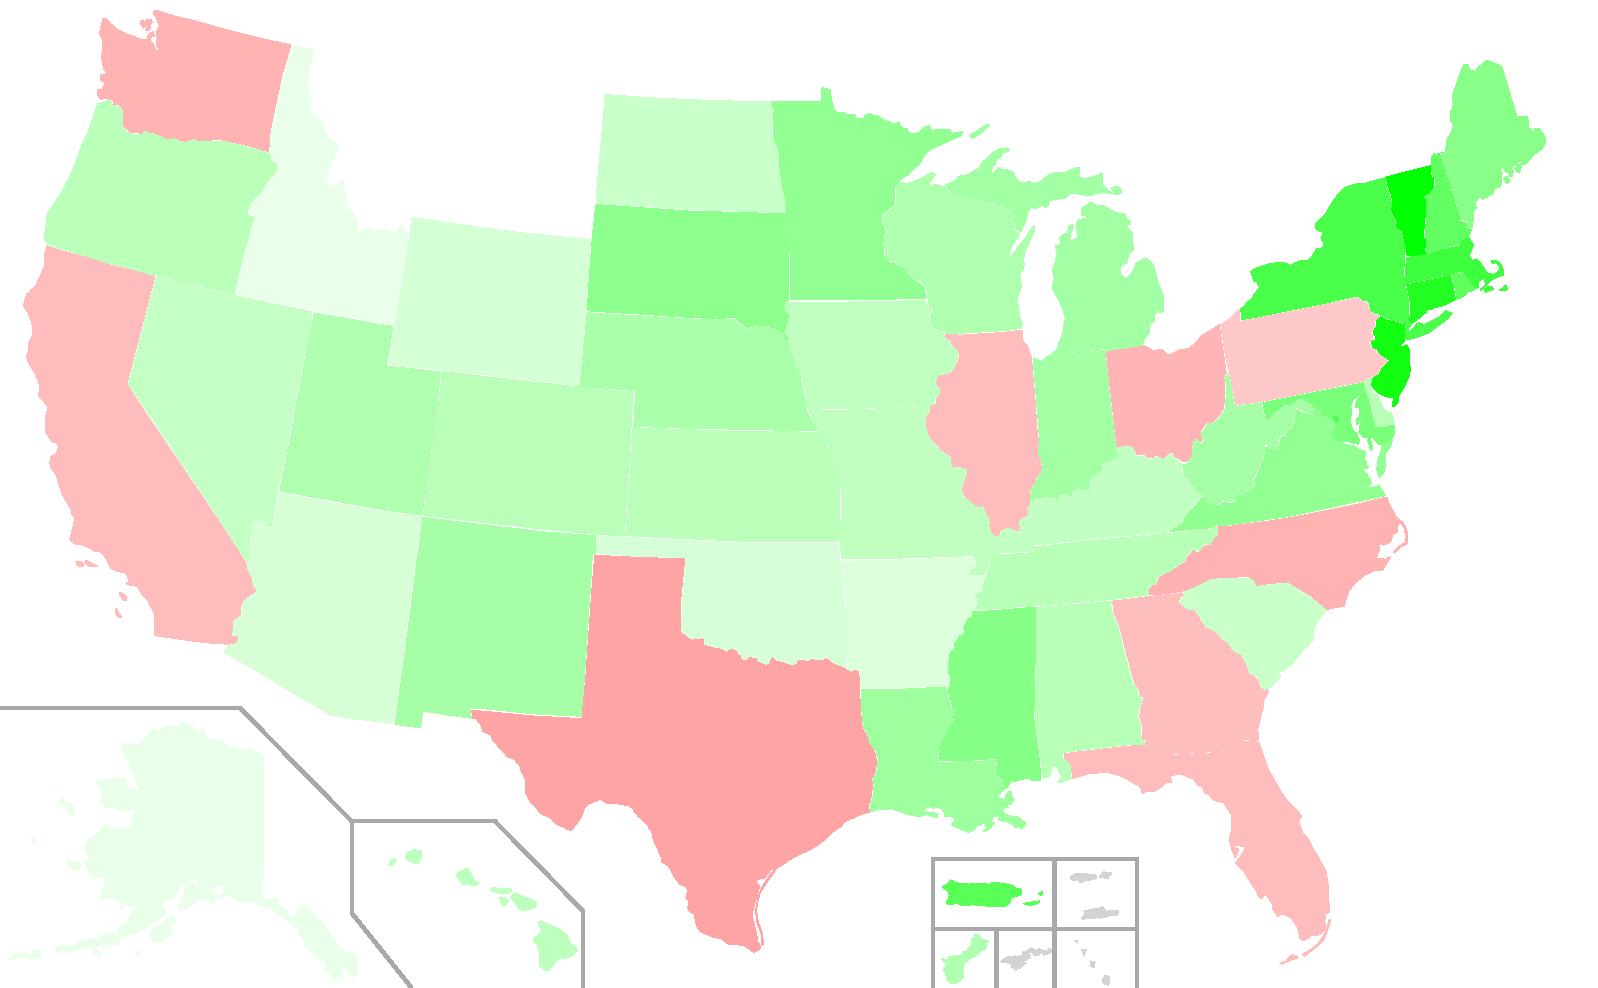
\includegraphics[width=53mm]{./images/ny.pdf}
\caption{Followers of New York}
\label{fig:state-ny}
\end{minipage}
\end{figure*}

\begin{figure*}[t]
\begin{minipage}[b]{0.32\linewidth}
\centering
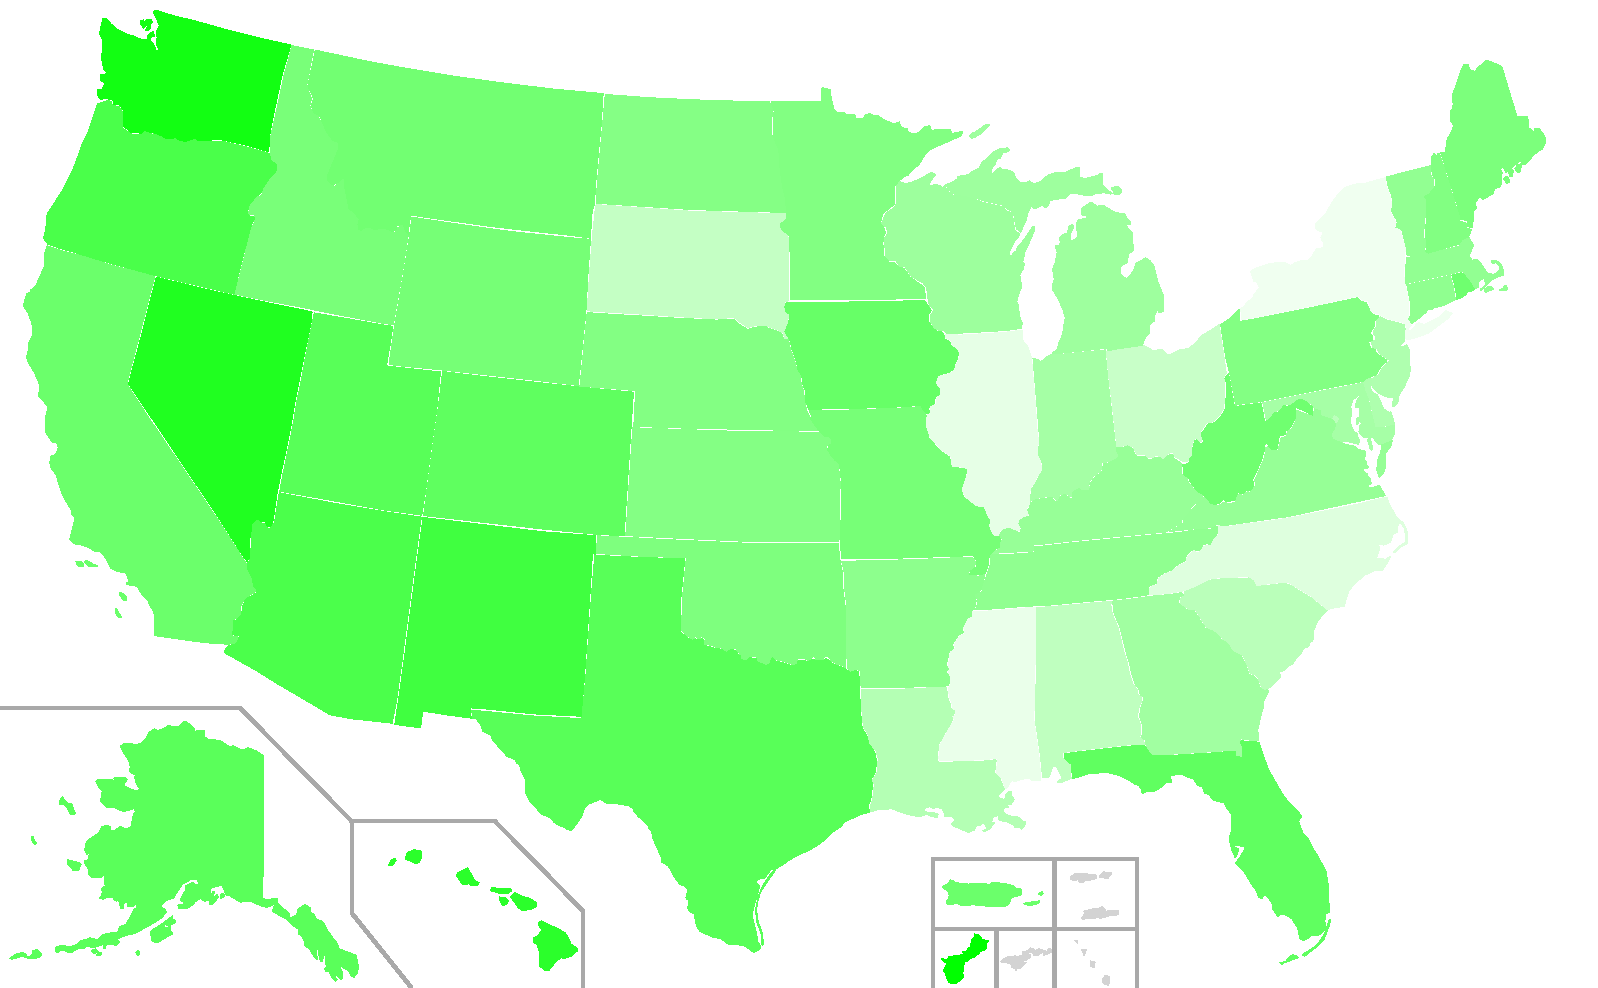
\includegraphics[width=53mm]{./images/fl.pdf}
\caption{Followers of Florida}
\label{fig:state-fl}
\end{minipage}
\hspace{2mm}
\begin{minipage}[b]{0.32\linewidth}
\centering
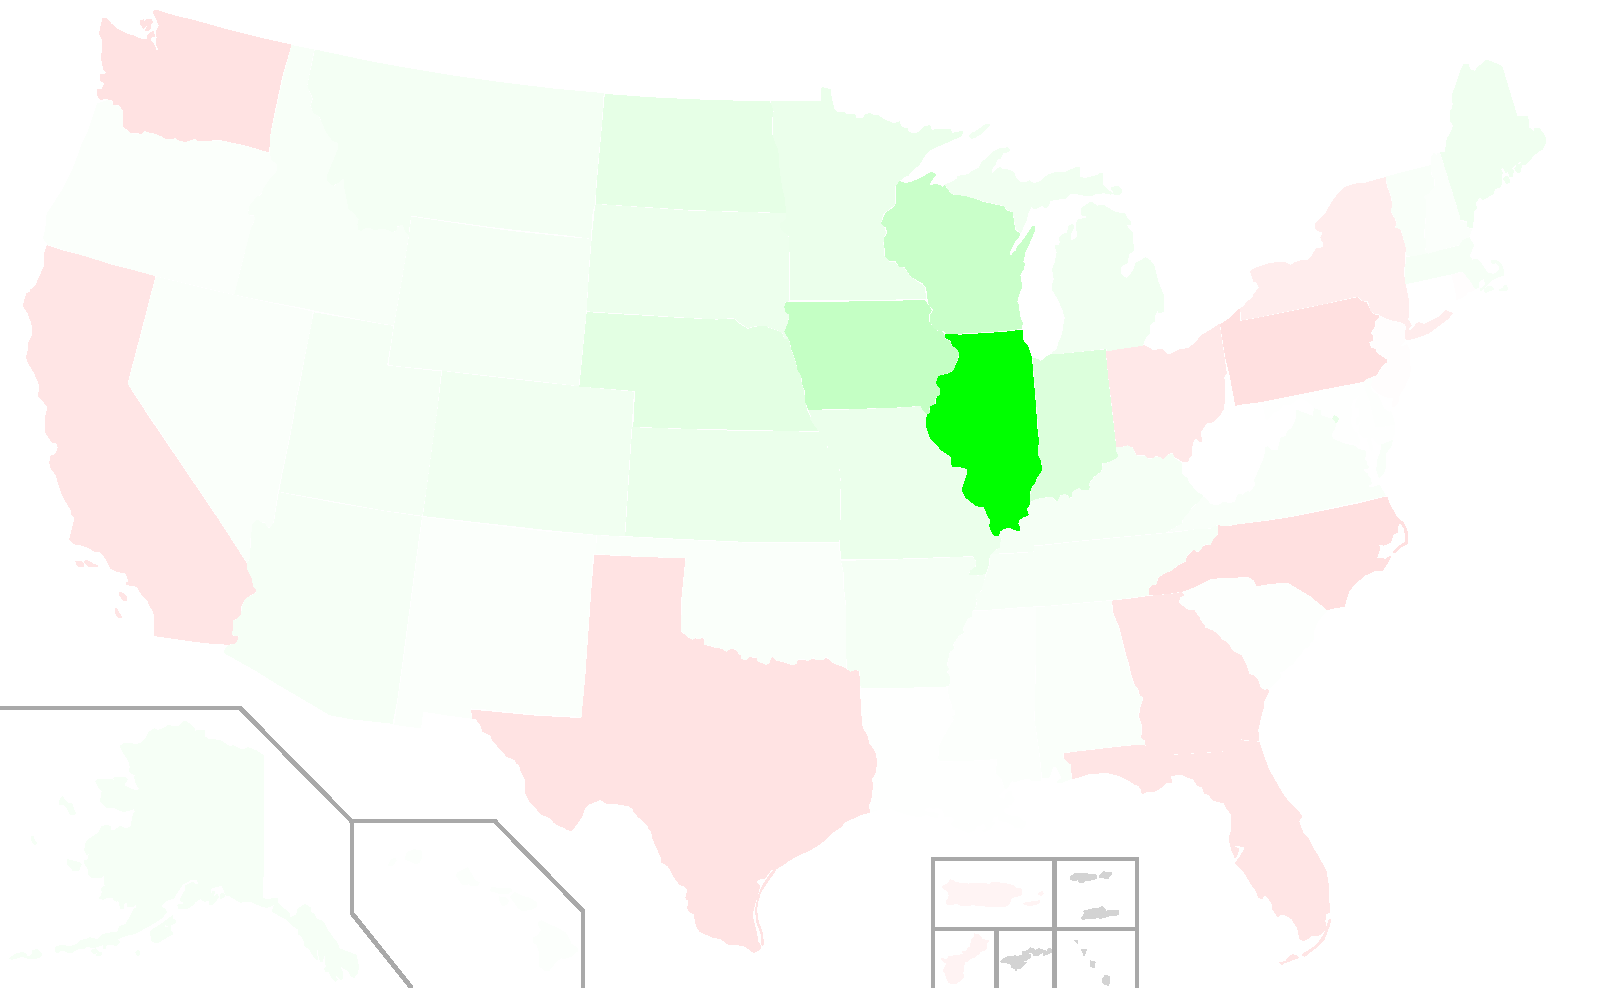
\includegraphics[width=53mm]{./images/il.pdf}
\caption{Followers of Illinois}
\label{fig:state-il}
\end{minipage}
\hspace{2mm}
\begin{minipage}[b]{0.32\linewidth}
\centering
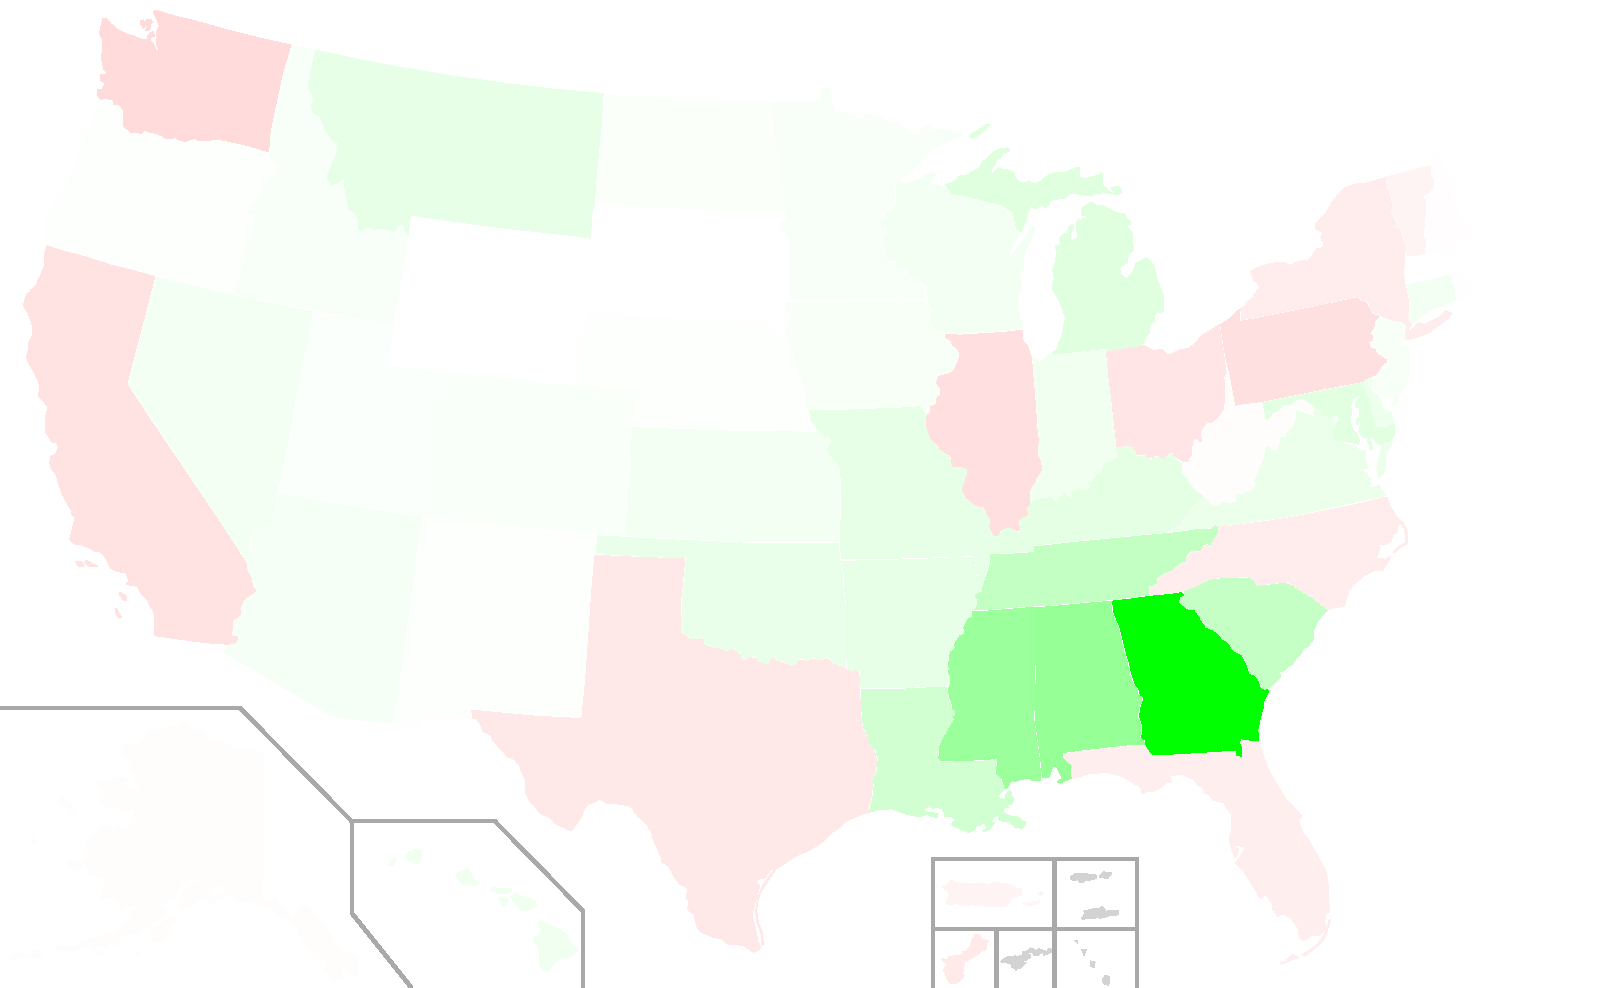
\includegraphics[width=53mm]{./images/ga.pdf}
\caption{Followers of Georgia}
\label{fig:state-ga}
\end{minipage}
\end{figure*}

\begin{figure*}[t]
\begin{minipage}[b]{0.32\linewidth}
\centering
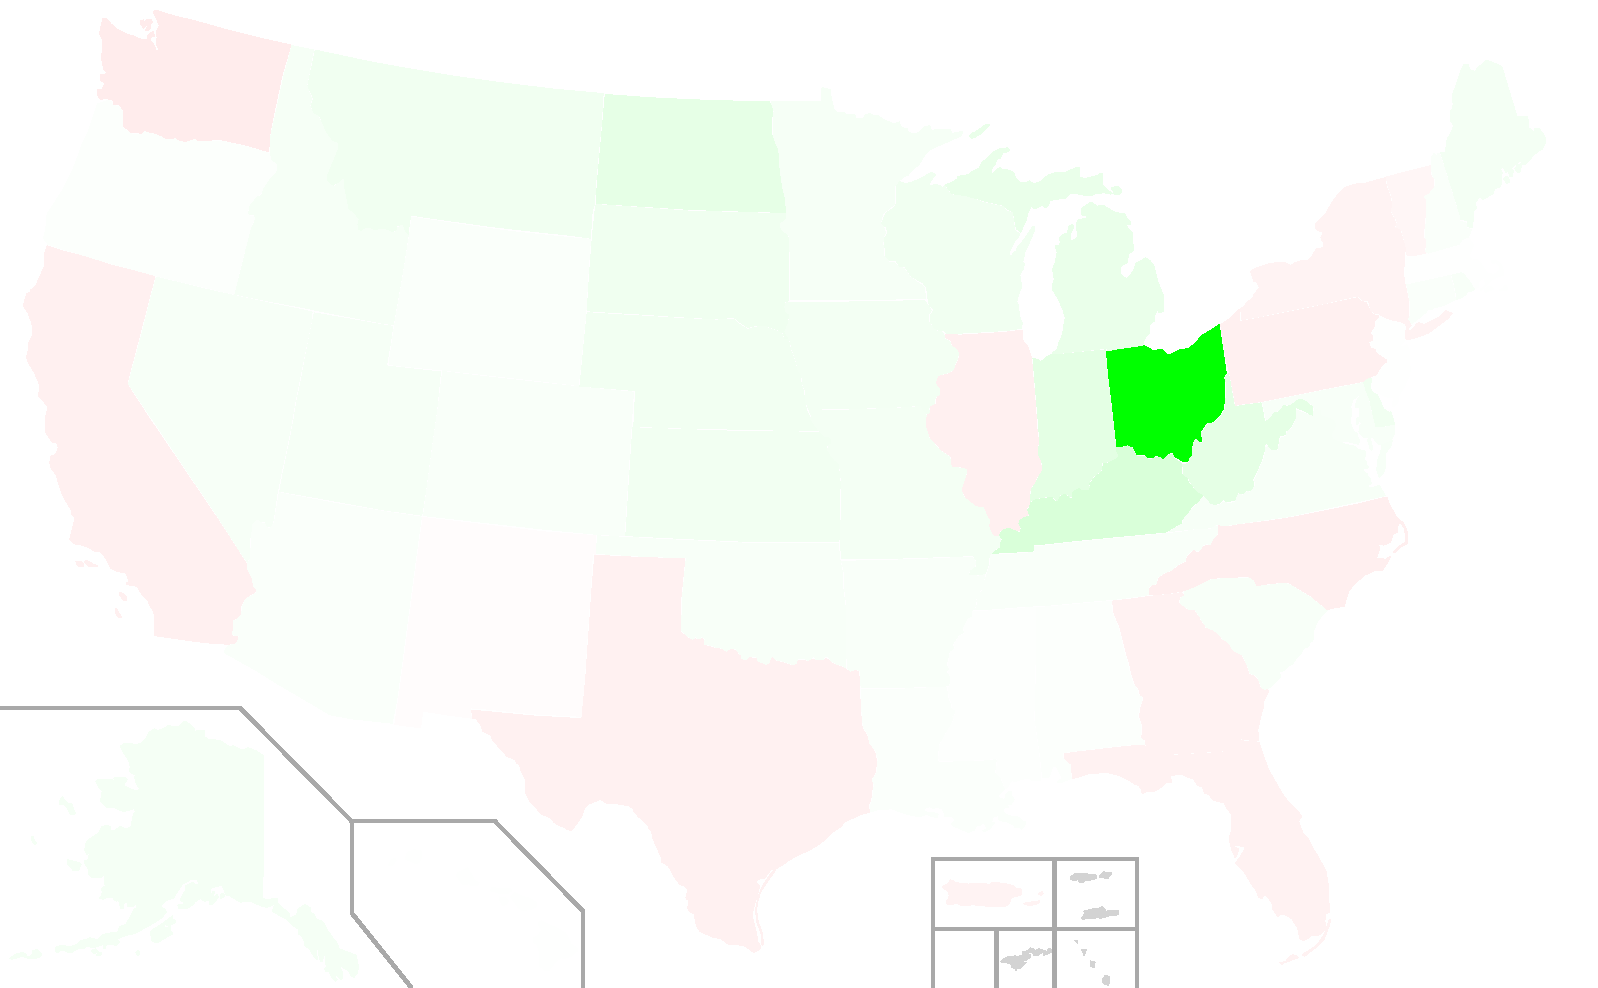
\includegraphics[width=53mm]{./images/oh.pdf}
\caption{Followers of Ohio}
\label{fig:state-oh}
\end{minipage}
\hspace{2mm}
\begin{minipage}[b]{0.32\linewidth}
\centering
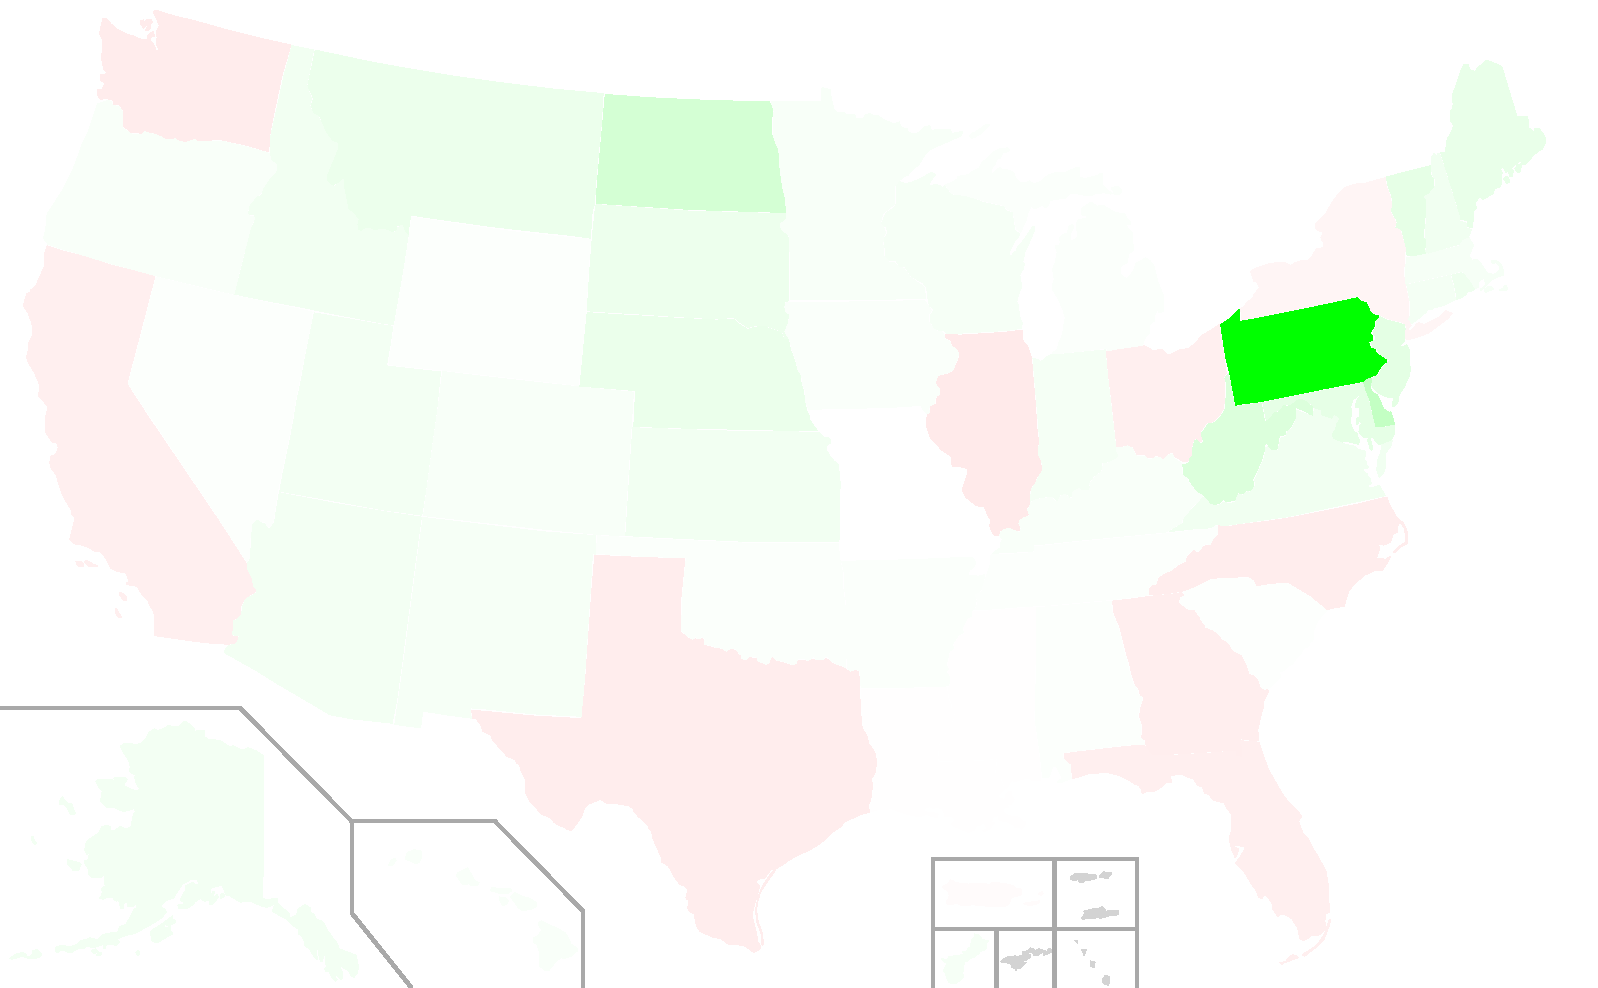
\includegraphics[width=53mm]{./images/pa.pdf}
\caption{Followers of Pennsylvania}
\label{fig:state-pa}
\end{minipage}
\hspace{2mm}
\begin{minipage}[b]{0.32\linewidth}
\centering
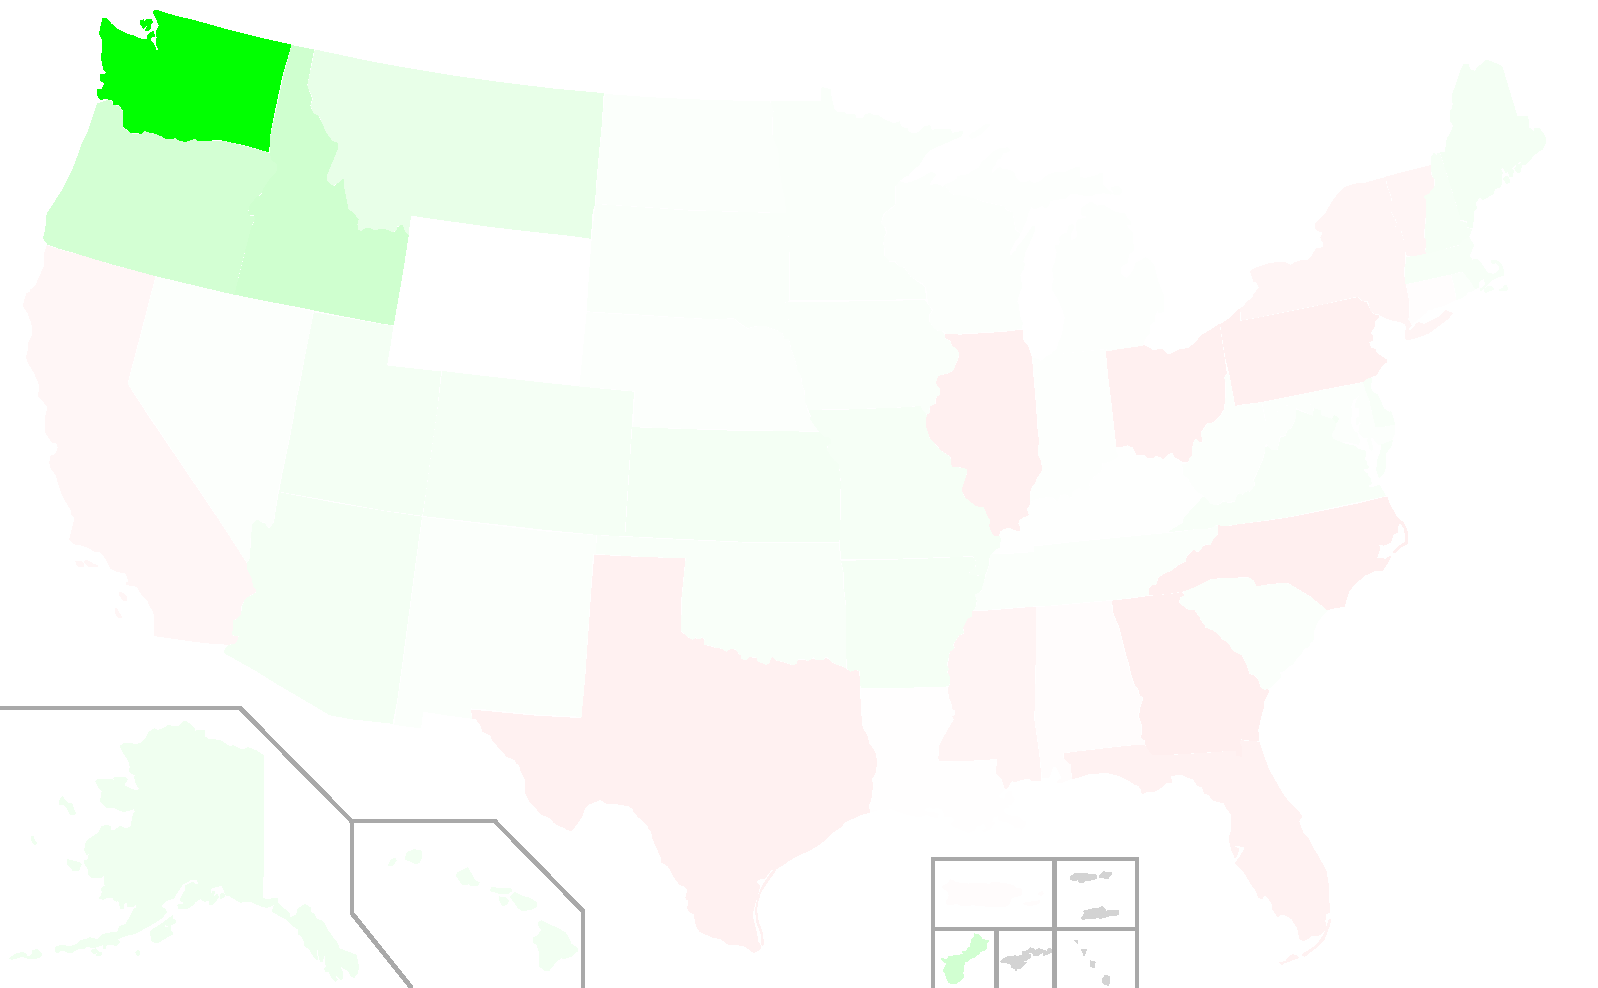
\includegraphics[width=53mm]{./images/wa.pdf}
\caption{Followers of Washington}
\label{fig:state-wa}
\end{minipage}
\end{figure*}

\begin{center}
\begin{figure*}[t]
\begin{minipage}[b]{0.32\linewidth}
\centering
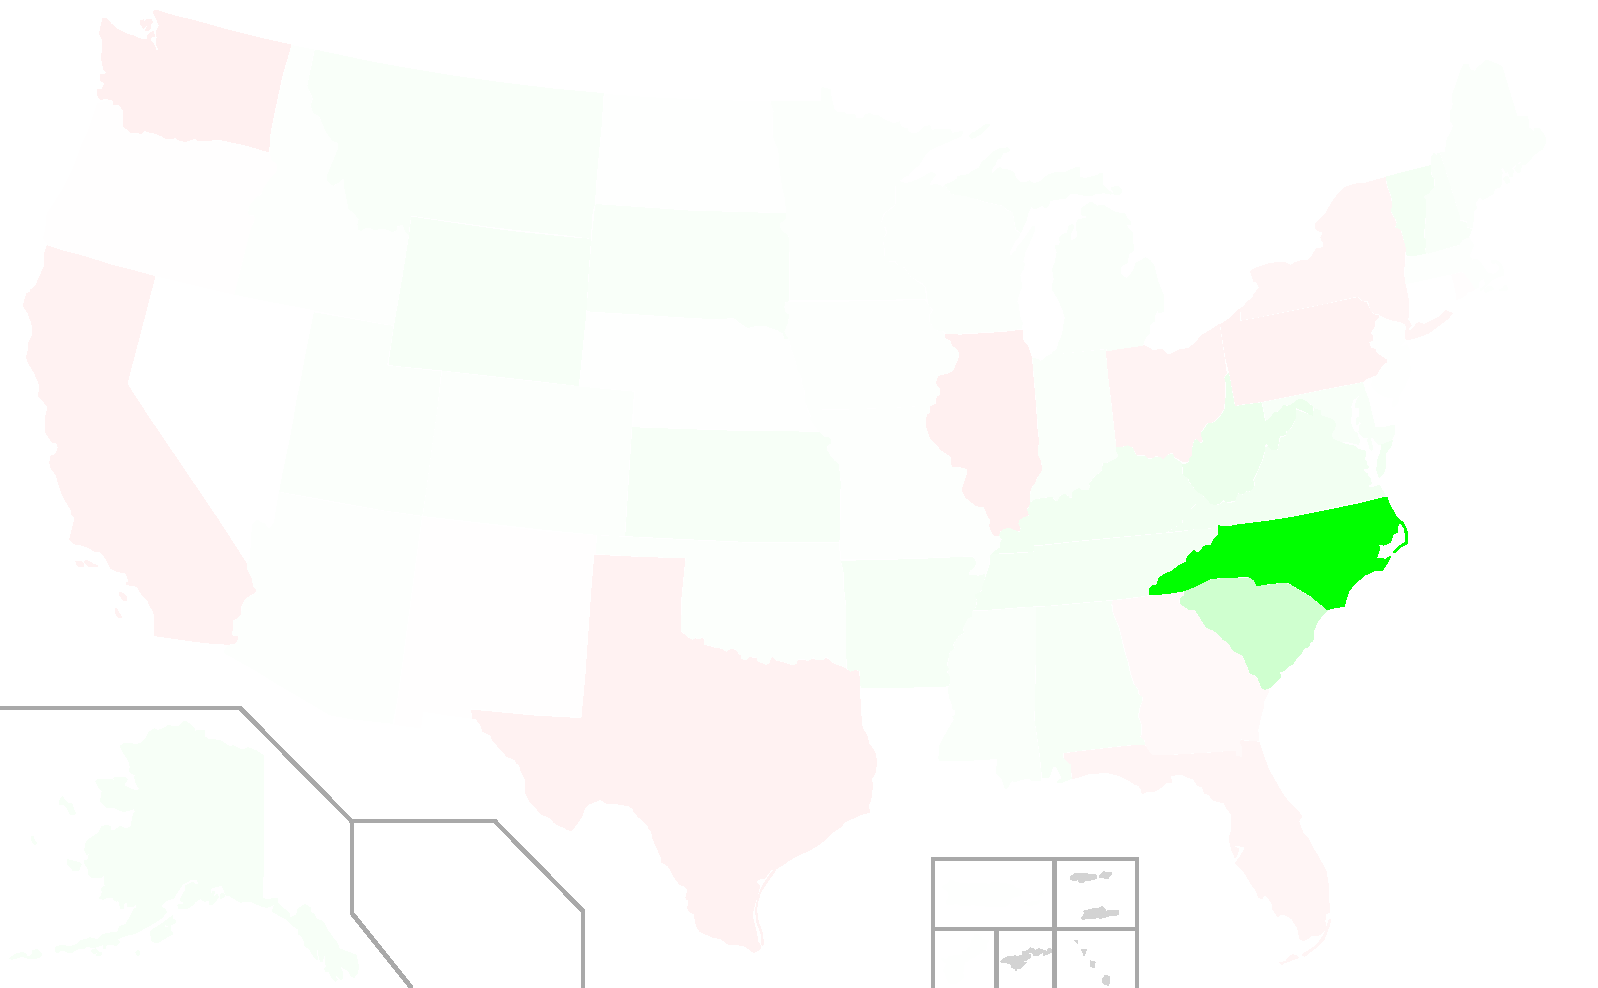
\includegraphics[width=53mm]{./images/nc.pdf}
\caption{Followers of North Carolina}
\label{fig:state-nc}
\end{minipage}
\end{figure*}
\end{center}

Our results are visualized for each attribute in figures throughout this paper.  These figures can be interpretted as follows: the groupings that are orderd by row are following the groupings that are ordered by column.  To read the bias for a particular relationship in these charts, find the desired row grouping and move right across the page.  Negative bias relationships are shaded red, and indicate that a row group has a bias against following a particular column group.  Positive bias relationships are shaded green, and indicate that a row group is biased in favor of following a particular column group.  The shade color increases with the strength of the bias.  Relationships that were not contained in our dataset are represented by gray-shaded empty squares.  For the sake of readability, the strength of shading is adjusted across different figures.  The strength of observed biases across different attributes is evaluated in \ref{sub:crossattribute}

Figure 6, a visualization of bias across follower count groupings, reveals a number of interesting facets of our Twitter subgraph.  One important feature is the values on the diagonal line moving from the top left to botthom right corner of the graph.  This line marks a group's affinity towards following itself, and will be referred to often in this section.  Here, we observe that our groupings are either neutral or subtly positively biased in favor of following their own group until a very high degree is reached.  The other exception to this trend is at the lowest follower count level, where the group is biased against following itself.  Across our results for the quantitative attributes it can be observed that users of extremely low degree exhibit unique behavior.

\begin{figure*}[t]
 \centering
 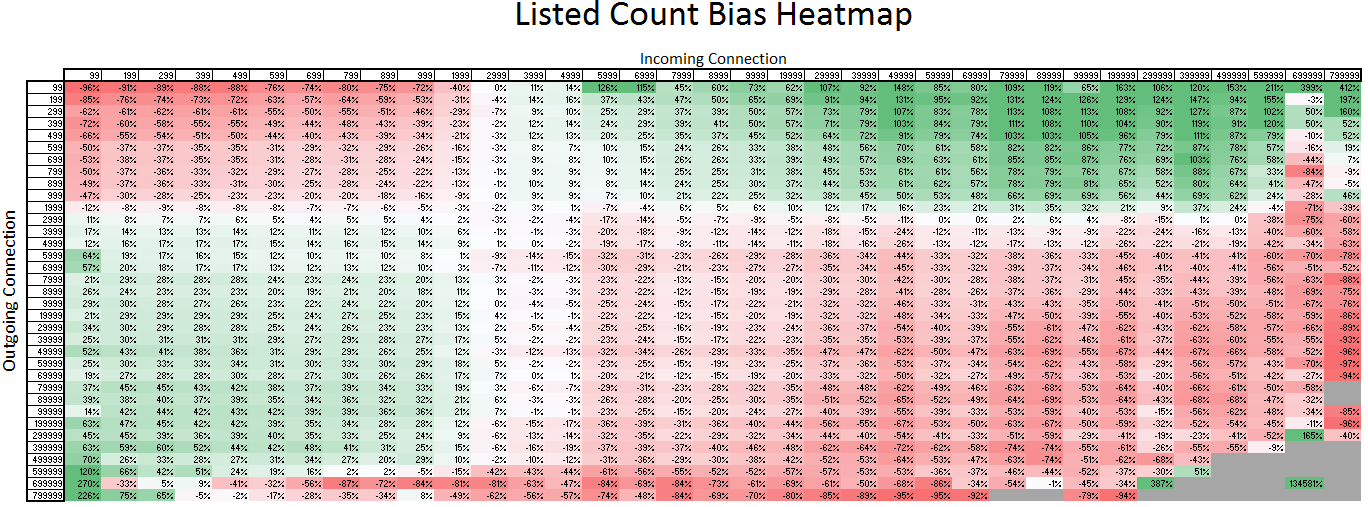
\includegraphics[bb=0 0 1026 380, scale=.3]{./images/Bates-Final/listedcount.png}
 % listedcount.png: 1368x507 pixel, 96dpi, 36.20x13.42 cm, bb=0 0 1026 380
 \label{fig:listed_count}
 \caption{A connectivity bias chart for number of lists a user appears on in logarithmically increasing groupings.}
\end{figure*}

Figure 7, a visualization of bias for the friend count attribute, contains much of the same trends that are observed in Figure 6.  A moderate bias towards following users of a similar friend count is clearly visible here along the chart's diagonal.  This bias grows stronger once the grouping being followed reaches a degree of greater than 2000, at which point there is extremely strong bias in favor of following users from these groups.  Unlike with follower count, low degree users follow eachother at a frequency above that which would be expected in an unbiased network.

Figure 8 displays bias patterns for user groupings by status count.  Our intuition here was that users would be that likely to connect to user accounts with different degrees of status count.  This intuition is at least partially confirmed in the graph -- low degree users are moderately biased towards following those with a high status count degree.  Those with a moderate-to-high status count are strongly biased against following others of a moderate-to-high status count.  This could be explained by businesses and professionals who use their twitter accounts to send frequent messages, but who follow very few people.

Figure 9 displays attribute relationships for users in different parts of the world by their offset from coordinated universal time.  While, UTC Offset generally refers to a longitudinal slice of the globe, certain offsets are used exclusively by certain countries or regions.  We observe that the strongest positive bias in this chart is at UTC Offset +5.5 following UTC Offset -8.  These two offsets correspond to user accounts in India and Sri Lanka following user accounts in Pacific Standard Time.  All groupings displayed varying degrees of bias against following user accounts at UTC Offset +9, which corresponds to the time zone in Japan and North and South Korea.  However, many of these groupings are not very well supported by our dataset.  We do not perform any further analysis on UTC offset.

Figures \ref{fig:state-ca}-\ref{fig:state-nc} show connectivity bias for the top 10 U.S. states, within the set of edges going to or coming from those states.  In general, states show a tendancy towards following themselves, and are followed by bordering states.  In the case of California, all states except the remaining top 9 are biased toward following California.  The mostly consistent bias against followers from the top 10 states is likely due to their being central to this analysis.

Figure 20 displays connectivity bias based on the number of Twitter lists that a user appears on.  Lists are a way to organize and separate different message streams, and our intuition here was that there would be a bias towards following users that appear more frequently on lists.  This trend is only strongly present for users with a low listed count following users with a high listed count.  Interesting, users of a high listed count display a moderate bias towards users of a low listed count.  High degree listed count users display a consistent moderate bias against following one another.

Figure 20(a) displays bias based on the user's system age in the Twitter network.  We observe a weak bias towards these groups following themselves until the oldest Twitter users are reached.  At this point, there is an extremely strong connectivity bias amongst these peers.  This is the most consistently strong bias that we observed in this report.  It should also be noted that there is a weak bias against new users following old users and vice versa.

Figure 20(b) displays bias across accounts of different language settings.  In our arrogance, the writers' intuition was that there would be a strong bias towards Twitter users following those of the English language setting.  Far from it, other language groupings besides English exhibit very strong bias towards following themselves.

Figure 20(c) displays connectivity bias based on whether or not a user's messages are protected.  The only considerable bias displayed in this chart is that users with protected accounts are biased against following one another.  Figure 20(d) displays significant positive bias for all relationships featuring non-geoenabled user groupings as well as a negative bias for \textit{Geoenabled follows Geoenabled}.


\begin{figure}[t]
 \centering
 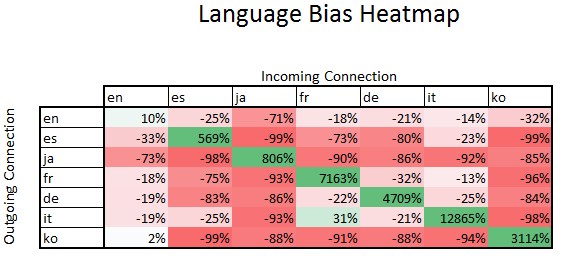
\includegraphics[bb=0 0 424 194, scale=.5]{./images/Bates-Final/lang.png}
 % lang.png: 565x259 pixel, 96dpi, 14.95x6.85 cm, bb=0 0 424 194
 \caption{A connectivity bias chart for users by language setting.}
 \label{fig:lang}
\end{figure}

\begin{figure}[t]
 \centering
 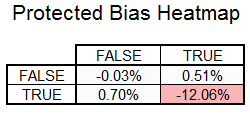
\includegraphics[bb=0 0 188 86, scale=.5]{./images/protected.png}
 % protected.png: 250x114 pixel, 96dpi, 6.62x3.02 cm, bb=0 0 188 86
 \caption{A connectivity bias chart for whether or not the user's account is protected.}
 \label{fig:protected}
\end{figure}

\begin{figure}[t]
 \centering
 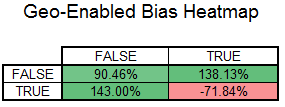
\includegraphics[bb=0 0 214 80, scale=.5]{./images/geoenabled.png}
 % geoenabled.png: 285x107 pixel, 96dpi, 7.54x2.83 cm, bb=0 0 214 80
 \caption{A connectivity bias chart for whether or not the user's account is geo-enabled to include location information with each tweet.}
 \label{fig:geoenabled}
\end{figure}

\subsection{Comparing Bias Across Different Attributes}
\label{sub:crossattribute}
While analyizing each attribute, we indentified several recurring bias patterns through which the attributes can be compared.  Each attribute can be described by its behavior across these bias patterns.  Across all attributes, we observed \textit{group follows itself} and \textit{group follows others} patterns.  There are additional patterns for attributes of continuous range -- \textit{low degree follows low degree}, \textit{high degree follows high degree}, \textit{low degree follows high degree}, and \textit{high degree follows low degree}.

We have characterized the strength of each of these bias patterns across all attributes.  For the sake of brevity, these have been summarized as a table in appendix \label{app:table_cross_attribute}.  Rather than mathematically define each bias pattern, we have decided to keep our identifications loose and use our visualizations as a guide.  The transition 'low degree' and 'high degree' is clear in the visual aids; the included table serves only as guide to compare the relative strengths of patterns in different attributes.